\documentclass[
	xcolor=dvipsnames,
	handout
]{beamer}

\usetheme{zhaw}

\usepackage{nameref}
\usepackage{amssymb}
\usepackage{amsmath}

\usepackage[utf8]{inputenc}
\usepackage[T1]{fontenc}

\usepackage{tabularx,colortbl}
\usepackage{xcolor}
\usepackage{listings}
\usepackage{upquote}
\usepackage{url}
\usepackage{etoolbox}
\usepackage{graphicx}
\usepackage{synttree}
\usepackage{listings}
\usepackage{multicol}
\usepackage{nopageno}

\definecolor{gray_ulisses}{gray}{0.55}
\definecolor{castanho_ulisses}{rgb}{0.71,0.33,0.14}
\definecolor{preto_ulisses}{rgb}{0.41,0.20,0.04}
\definecolor{green_ulises}{rgb}{0.2,0.75,0}

\definecolor{background}{RGB}{240, 240, 190}
\definecolor{string}{RGB}{230, 219, 116}
\definecolor{comment}{RGB}{117, 113, 94}
\definecolor{normal}{RGB}{248, 248, 242}
\definecolor{identifier}{RGB}{166, 226, 46}

\lstdefinelanguage{Golang}{
	morekeywords=[1]{package,import,func,type,struct,return,defer,panic,recover,select,var,const,iota},
	morekeywords=[2]{string,uint,uint8,uint16,uint32,uint64,int,int8,int16,int32,int64,bool,float32,float64,complex64,complex128,byte,rune,uintptr,error,interface},
	morekeywords=[3]{map,slice,make,new,nil,len,cap,copy,close,true,false,delete,append,real,imag,complex,chan},
	morekeywords=[4]{for,break,continue,range,go,goto,switch,case,fallthrough,if,else,default},
	morekeywords=[5]{Println,Printf,Error,Print},
	sensitive=true,
	morecomment=[l]{//},
	morecomment=[s]{/*}{*/},
	morestring=[b]',
	morestring=[b]",
	morestring=[s]{`}{`},
}
\lstdefinestyle{basestyle}{
	basicstyle=\small\ttfamily,
	breakatwhitespace = true,
	tabsize = 4,
	frame = double,
%	numbers = left,
	numbersep = 10pt,
%	numberstyle = {\tiny\emptyaccsupp},
%	firstnumber = auto,
	numberblanklines = true,
	captionpos = b,
	columns = fullflexible,
	extendedchars = true,
	float = ht,
	showtabs = false,
	showspaces=false,
	showstringspaces=false,
	breaklines=true,
%	prebreak=\Righttorque
	backgroundcolor=\color{background!40!white},
	keywordstyle=\color{blue!70!castanho_ulisses}\bfseries,
	commentstyle=\color{green!50!castanho_ulisses}\ttfamily,
%	morekeywords={printstr, printhexln},
	stringstyle=\color{red!70!castanho_ulisses},
	xleftmargin = \fboxsep,
	xrightmargin = -6pt,
	showstringspaces=true,
}

\newenvironment{zhawframe}[1][]
{\begin{frame}[environment=fr,#1]{\insertsubsectionhead}{\insertsectionhead}}
{\end{frame}
}

\setbeamertemplate{footline}[frame number]

\title{Design and Implementation of an Alternative to SSH}
\date{\today}
\author{Raphael Emberger}

\begin{document}
\maketitle

%\section*{Index}
%\begin{zhawframe}[shrink]
%\begin{multicols}{2}
%\tableofcontents
%\end{multicols}
%\end{zhawframe}

\section{The Problem}
\begin{zhawframe}
\onslide<1-> Design and implement an alternative to \textcolor{red}{SSH} (prototype)

\onslide<2-> Implementation language: \textcolor{red}{Go} (Golang)

\onslide<3-> Target platform: \textcolor{red}{GNU/Linux}
\end{zhawframe}

\section{The Present Solution}
\subsection{Telnet}
\begin{zhawframe}
\onslide<1-> \textcolor{red}{telnet(1) is old} (RFC15 1969, RFC854 1983)

\onslide<2-> \textcolor{red}{No secure connection} (except: TELNETS)

\onslide<3-> "Go-Telnet"
\end{zhawframe}

\subsection{Berkeley \texttt{r}-Commands}
\begin{zhawframe}
Frequently used Linux commands made into \texttt{r}-Commands:
\begin{itemize}
\item \texttt{login}(1) $\Rightarrow$ \texttt{\textcolor{red}{r}login}(1)
\item \texttt{sh}(1)/\texttt{bash}(1) $\Rightarrow$ \texttt{\textcolor{red}{r}sh}(1)/\texttt{\textcolor{red}{r}exec}(1)*
\item \texttt{cp}(1) $\Rightarrow$ \texttt{\textcolor{red}{r}cp}(1)
\item \texttt{who}(1) $\Rightarrow$ \texttt{\textcolor{red}{r}who}(1)
\item \texttt{stat}(1) $\Rightarrow$ \texttt{\textcolor{red}{r}stat}(1)
\item \texttt{uptime}(1) $\Rightarrow$ \texttt{\textcolor{red}{r}uptime}(1)
\end{itemize}
Useful (especally for scripts), but \textcolor{red}{no secure connection}
\end{zhawframe}

\subsection{OpenSSH}
\begin{zhawframe}
\onslide<1-> Replaces telnet(1) and Berkeley \texttt{r}-commands

\onslide<2-> \textcolor{red}{Secure connection} (own protocol)

\onslide<3-> Plethora of features:
	\begin{itemize}
	\item<3-> Remote user login
	\item<3-> Auth via keys
	\item<3-> Port forwarding
	\item<3-> X11-forwarding
	\item<3-> Auth agent connection forwarding (!)
	\item<3-> Compression (used by \texttt{rsync}(1))

	\hspace{3mm}$\vdots$
	\end{itemize}
\end{zhawframe}

\section{My Solution}
\subsection{Secure Connection}
\begin{zhawframe}
\onslide<1-> \textcolor{red}{Prevent MITM, provide integrity \& privacy}

\onslide<2-> TLS 1.3

\onslide<3-> Server: \texttt{openssl}(1) $\rightarrow$ key \& X.509 certificate

\onslide<4-> \texttt{crypto/tls}

\onslide<5-> \textcolor{red}{Encrypted channel}

\onslide<6-> Self signed server certificate: Ignores trust chain

\onslide<7-> No client certificates (!) \onslide<8->$\rightarrow$ Cannot authenticate the connecting client
\end{zhawframe}

\subsection{Authentication via Password}
\begin{zhawframe}
\onslide<1-> \texttt{/etc/passwd} (!)

\onslide<2-> \textcolor{red}{PAM}

\onslide<3-> No Go-package for PAM

\onslide<4-> Failure in test environment $\rightarrow$ \textcolor{red}{\texttt{login}(1)}

\onslide<5-> Failure in same environment using \texttt{login}(1)

\onslide<5-> Too time consuming to switch back

\onslide<6-> \texttt{login}(1) allows root login

\onslide<7-> Prefetch credentials on client
\end{zhawframe}

\subsection{Authentication via Keys}
\begin{zhawframe}
\onslide<1-> Authenticate via \textcolor{red}{public key cryptography}

\onslide<2-> Store authorized public keys on server

\onslide<3-> Authorized keys stored in \texttt{/root/.gosh} (plain-text)

\onslide<4->$\quad\rightarrow$ \textcolor{red}{Hash in \texttt{\textasciitilde{}/.gosh/authorized\_{}keys}}

\onslide<5->$\quad\rightarrow$ Important for privilege separation
\end{zhawframe}

\subsection{Privilege Separation}
\begin{zhawframe}
\onslide<1-> Shell should run with \textcolor{red}{appropriate permissions} (\texttt{setuid}(2)/\texttt{setgid}(2))

\onslide<2-> Failure to \textcolor{red}{drop privileges} after login (operation not \textcolor{red}{supported})

\onslide<4-> $\quad$ Thank you, Go \onslide<5->$\rightarrow$ spawn shell with appropriate UID \& GID

\onslide<6-> SSH more sophisticated
\end{zhawframe}

\begin{zhawframe}
\begin{figure}[ht]
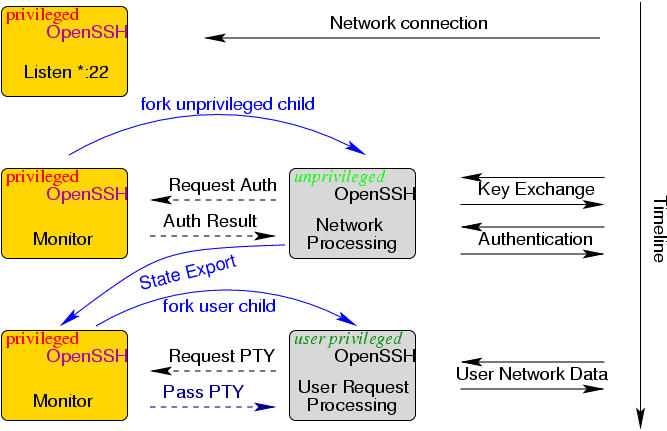
\includegraphics[width=\textwidth]{priv}
\end{figure}
\end{zhawframe}

\subsection{Forking}
\begin{zhawframe}
\begin{itemize}
\item<1-> Server spawns child to handle connection
\item<2-> \texttt{fork}(2)
\item<3-> Go: \textcolor{red}{No support for forking}
\item<4-> CGO fork fails
\item<5-> \texttt{syscall.ForkExec}

\onslide<6->$\rightarrow$ High level connection object gets corrupted
\item<7-> \textcolor{red}{Create host application}
\item<8-> \textcolor{red}{Transfer \texttt{fd}} as argument to child

\onslide<9->$\rightarrow$ Low level socket from \texttt{x/sys/unix} (x-package!)
\item<10-> Prospect: Implement proper privilege separation
\end{itemize}
\end{zhawframe}

\subsection{Login Accounting}
\begin{zhawframe}
\onslide<1-> Not implemented, \textbf{but}

\onslide<2-> \textcolor{red}{\texttt{utmpx}} $\rightarrow$ \texttt{w}/\texttt{who}

\onslide<3-> \textcolor{red}{PAM}: \texttt{pam\_{}open\_{}session}(3)/\texttt{pam\_{}close\_{}session}(3)
\end{zhawframe}

\subsection{User Data Acquisition}
\begin{zhawframe}
\onslide<1-> Home directory, shell, UID \& GID

\onslide<2-> Go standard library incomplete (misses shell information)

\onslide<3-> \texttt{/etc/passwd} (!) $\Rightarrow$ \textcolor{red}{CGO: \texttt{getpwnam}(2)/\texttt{getpwuid}(2)}
\end{zhawframe}

\subsection{Pseudoterminals}
\begin{zhawframe}
Shells expect to be connected to a \textcolor{red}{TTY}
\begin{figure}[ht]
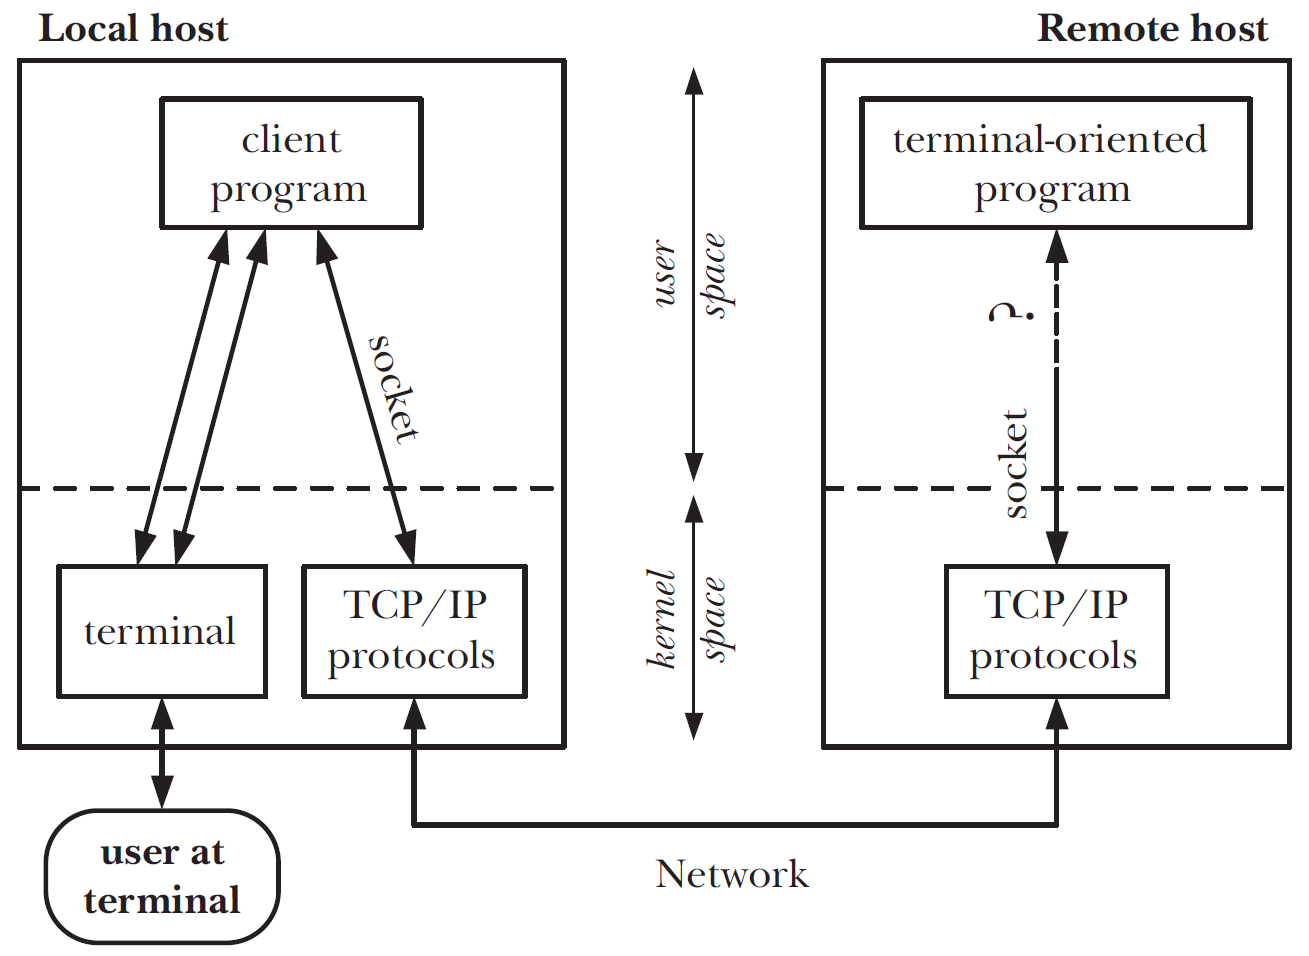
\includegraphics[width=0.8\textwidth]{PseudoterminalProblem}
\end{figure}
\end{zhawframe}

\begin{zhawframe}
\textcolor{red}{PTY} fakes being a TTY
\begin{figure}[ht]
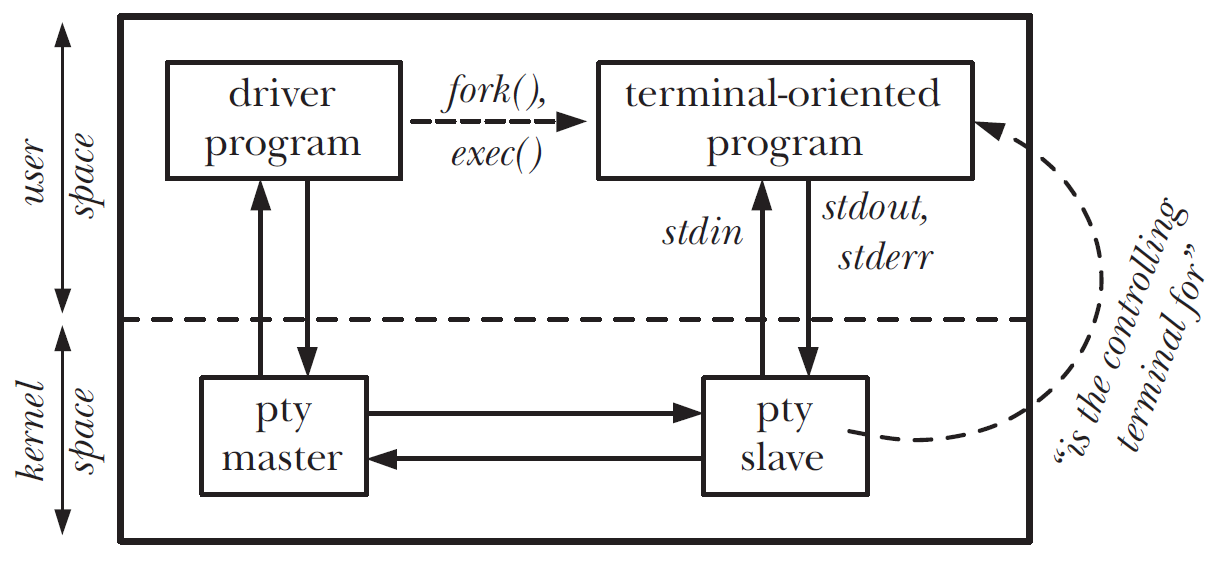
\includegraphics[width=0.94\textwidth]{Pseudoterminal}
\end{figure}
\end{zhawframe}

\begin{zhawframe}
Overview
\begin{figure}[ht]
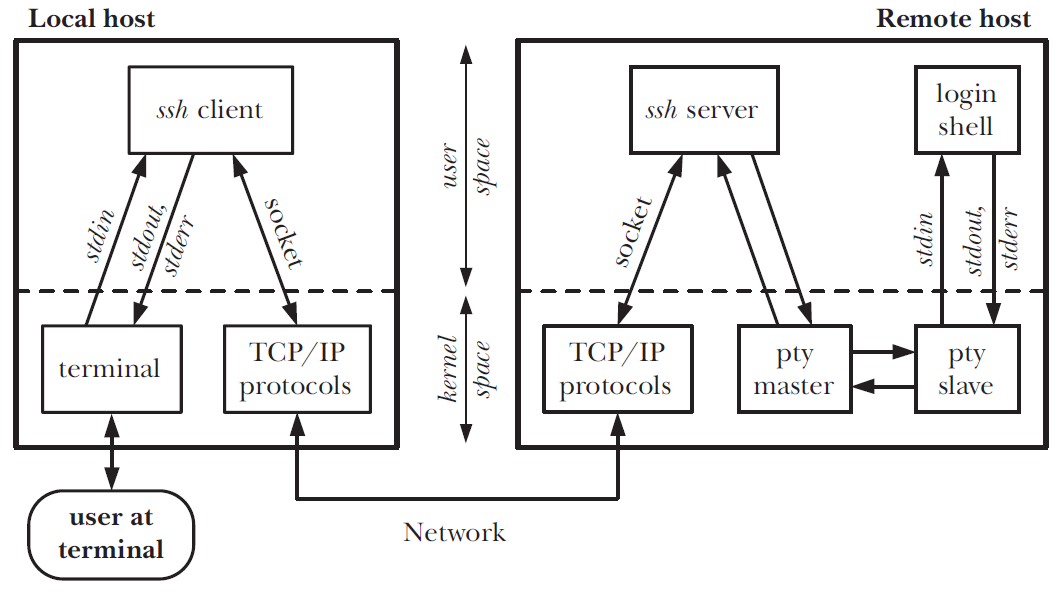
\includegraphics[width=0.85\textwidth]{PseudoterminalSSH}
\end{figure}
\end{zhawframe}

\begin{zhawframe}
\onslide<1-> \textcolor{red}{\texttt{istty}(3)} on the connected \texttt{fd}s

\onslide<2-> \texttt{posix\_{}openpt("/dev/ptmx")}(3) $\rightarrow$ \texttt{grant\_{}pt}(3) $\rightarrow$ \texttt{unlockpt}(3) $\rightarrow$ \texttt{ptsname}(3)

\onslide<3-> \textcolor{red}{Wrapper function in} internal(!) package of the \textcolor{red}{Go standard library} \texttt{os/signal/internal/pty}
\end{zhawframe}

\subsection{Starting the Shell}
\begin{zhawframe}
\onslide<1-> Shell requirements:

	\begin{itemize}
	\item user (\textcolor{red}{UID \& GID}) \& host name
	\item \textcolor{red}{\texttt{TERM}} env var (for \texttt{ncurses}(3X))
	\item \textcolor{red}{window resolution} (including \texttt{SIGWINCH})
	\item \textcolor{red}{session leader} (controlling terminal)
	\end{itemize}
	
\onslide<2-> \textcolor{red}{Transfer} of env vars (client $\leftrightarrow$ server)

\onslide<3-> Continuous transfer of \texttt{SIGWINCH} not implemented $\rightarrow$ prospects

\onslide<4-> Setting \texttt{CTTY} flag (for controlling terminal) fails $\rightarrow$ prospects
\end{zhawframe}

\subsection{Terminal Mode}
\begin{zhawframe}
\onslide<1-> \textcolor{red}{Forward all keystrokes} without interpretation (client-sside)

\onslide<2-> \texttt{cooked} mode $\rightarrow$ \textcolor{red}{\texttt{raw} mode}

\onslide<3-> x-package (!) \texttt{x/crypto/ssh/terminal}
\end{zhawframe}

\section{How It Turned Out}
\subsection{Performance}
\begin{zhawframe}
\onslide<1-> client \textcolor{green!60!blue}{$\leftrightarrow$} server $\leftrightarrow$ ptm $\leftrightarrow$ pts $\leftrightarrow$ shell

\onslide<2-> \texttt{/dev/zero} $\rightarrow$ connection (client-side) $\rightarrow$ server $\rightarrow$ \texttt{pv -rabtW} $\rightarrow$ \texttt{/dev/null}

\onslide<3-> TLS vs no TLS

\onslide<4->
\begin{table}[ht]
\centering
\begin{tabular}{rcc}
Throughput with:		& TLS (total)	& no TLS (size)\\\hline
Linux 					& 427MiB/s (25.1GiB)	& 1177.6MiB/s (69.0GiB)\\
WSL 					& 69.7MiB/s (4.09GiB)	& 116MiB/s (6.82GiB)\\
Linux to WSL (eth*) 	& \textcolor{red}{85.1MiB/s} (4.99GiB)	& \textcolor{red}{83.7MiB/s} (4.91GiB)
\end{tabular}
\end{table}
\onslide<4-> *: Netgear Switch \& Cat 5 ethernet cable
\end{zhawframe}

\subsection{Comparison to Telnet}
\begin{zhawframe}
\onslide<1-> TLS vs plain text

\onslide<2-> Key auth vs only password auth
\end{zhawframe}

\subsection{Comparison to Berkeley \texttt{r}-commands}
\begin{zhawframe}
\onslide<1-> Only \texttt{rlogin}(1) is considered (\texttt{rsh}(1))

\onslide<2-> TLS vs plain text

\onslide<3-> Key auth vs only password auth
\end{zhawframe}

\subsection{Comparison to OpenSSH}
\begin{zhawframe}
\onslide<1-> TLS vs own protocol

\onslide<2-> Privilege separation

\onslide<3-> Many additional features
\end{zhawframe}

\section{Afterthoughts}
\begin{zhawframe}
\onslide<1-> Many problems encountered

\onslide<2-> Many new concepts learned

\onslide<3-> Mixed feelings
\end{zhawframe}

\subsection{End}
\begin{zhawframe}
Thank you for your attention!
\end{zhawframe}
\end{document}